\chapter{DESIGN}
\begin{spacing}{1.5}
This new solution uses a combination of Microformats-style markup and RDFS to provide a comprehensive framework for describing, discovering and composing RESTful services by adding semantics. Microformats, being simple and reusing a lot of the properties of HTML, provides users with a low entry-barrier for developers, which can increase adoption rate. These annotations are not visible to user but hidden in the HTML source and hence do not come in the way of users browsing the site.

In order to enable strong interlinking between services, a more robust solution like RDF and a backing RDF Schema is needed. This is achieved by providing an adapter for automatic conversion from the Microformat to RDF and providing a ready-made RDF Schema for the purpose(Figure: \ref{fig:micro_vs_rdf}). This way, the developers need not be concerned with the RDF descriptions that work in the background.

The solution currently addresses RESTful services that represent resources using JavaScript Object Notation (JSON). It is possible to extend the idea to XML based services as well by making some assumptions about the XML serialization.

\begin{figure}
        \centering
        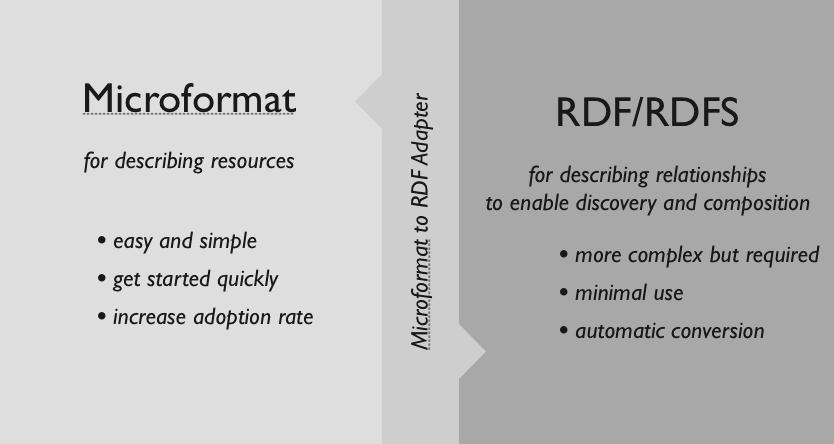
\includegraphics[scale=0.3]{images/micro_vs_rdf.png}
        \caption{Overview of the new architecture }
        \label{fig:micro_vs_rdf}
\end{figure}


\section{Service Description}

Services are described using special purpose annotations in the HTML code. These annotations are specified in the class attribute of the associated tags. This attribute is usually used for classification of HTML elements and also as selectors for JavaScript access and to style elements via CSS. Using special purpose annotations as class names help us to reuse whatever is already provided by HTML and JavaScript. Following annotations are proposed for describing resources in a RESTful API.

An intelligent agent extracts information about the service by traversing the DOM tree of the HTML page. APIs for traversing trees are available in almost all programming languages including JavaScript which is used extensively on the web and also to make extensions for many popular browsers such Chrome and Safari. Browsers or browser extensions could then could parse this data and automate the creation of clients for these services.


\section{Annotations}

Services are described using special purpose annotations in the HTML code. These annotations are specified in the class attribute of the associated tags.

\subsection{General Annotations}
\begin{enumerate}

\item {\bf hresource}: This is the root annotation that marks the resource description. All other annotations are contained within an element marked with class="hresource". A client parsing a page could treat the presence of this annotation as an indication of the existence of a resource description on the page. Unless all other annotations are encapsulated in an hresource, they will not be parsed.

\item {\bf name} :Annotates the name of the resource. This can be any human readable name and need not have any programming significance.

\item {\bf url/uri}: Annotates the URL at which the resource is accessible.
\end{enumerate}

\subsection{Annotation of Methods}
Annotates Permissiable methods (GET,POST,PUT,DELETE)

\begin{enumerate}
\item {\bf method}: This is the root annotation that marks the permissiable method. It contains following sub-annotations
\begin{itemize}
\item {\it type}: HTTP request type. GET,POST,PUT,DELETE
\item {\it input}:  (optional) input attribute
\item {\it output}: (optional) output attribute
\item {\it header}: (optional) attributes that should be passed as header to HTTP request
\end{itemize}
\end{enumerate}

\subsection{Annotation Of Attributes}
\begin{enumerate}
\item {\bf attribute}: Annotates an attribute/property of the resource. All attributes of a resource should be annotated with this annotation. Specific characteristics of the attribute could be further specified by more annotations that are used together with the attribute annotation.

\item {\bf required}: Indicates a required attribute. This annotation is always used along with the attribute annotation.

\item {\bf queryable}:  Indicates an attribute that may be provided in the HTTP querystring during a GET operation to filter the results. This annotation is always used along with the attribute annotation.

\item {\bf read-only}:  Indicates a read-only attribute. A read-only attribute may be retrieved during a GET operation but may not be included in a POST or a PUT. This annotation is always used along with the attribute annotation.write-once: Indicates a write-once attribute that can be specified only during the create operation (POST) but not during update (PUT). This annotation is always used along with the attribute annotation.

\item {\bf guid}: Indicates if an attribute is a globally unique identifier for the resource that could be used across multiple services.
\item {\bf Comment}: Provides a human-readable description of the attribute. This should be descendant of parent of attribute node

\item {\bf hresource-datatype}: Annotates the datatype of the attribute.This should be descendant of parent of attribute node.For permissible types see table: \ref{tab:data_types}

\begin{table}
    \centering
    \begin{tabular}{|l|l|}
    \hline
    Data Type      & Description                    \\ \hline
    Integer or Int &  32 bit integer                \\ \hline
    float          & floating point number          \\ \hline
    Int64          &  64 bit integer.               \\ \hline
     Range         &  Boolean or Bool               \\ \hline
    Date or Time   & should specify date formatting \\ \hline
    Timestamp      & Timestamp of entity            \\ \hline
    \end{tabular}
    \caption{Data types}
    \label{tab:data_types}
\end{table}

{\bf eg}: Range(0.0,1.0) specifies floating point number between 0 and 1 and Range(0,1) specifies integer between 0 and 1.
\end{enumerate}

\subsection{Annotation of Errors}

\begin{enumerate}
\item {\bf hresource-error}: This is the root annotation that marks the errors.It should contain two sub-annotation for each error:
\begin{itemize}
\item {\it error-code}:Specify the error code.
\item {\it comment}: Description of error.
\end{itemize}
\end{enumerate}
eg:
\begin{minted}{html}
<li class="hresource-error">
      <code class="error-code">201$</code>-<span class="comment">
      test failed</span>
      </li>
\end{minted}

The relationship between these sematnic annotataion is shown in figuere \ref{fig:rel_semantic} (hresource-produced-by and hresource-consumed-by are described in section \ref{sec:service_disc})
\begin{figure}
        \centering
        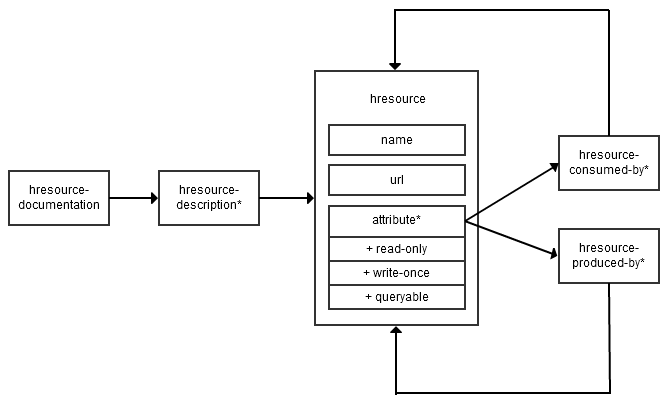
\includegraphics[scale=0.5]{images/rel_semantic.png}
        \caption{Relationship between the semantic annotations}
 ('*' indicates a one-to- many relationship)
        \label{fig:rel_semantic}
\end{figure}


An intelligent agent extracts information about the service by traversing the DOM tree of the HTML page(See figure \ref{fig:code}. APIs for traversing trees are available in almost all programming languages including JavaScript which is used extensively on the web and also to make extensions for many popular browsers such Chrome and Safari. Browsers or browser extensions could then could parse this data and automate the creation of clients for these services.

%include code.
\begin{figure}
\begin{minted}{html}

<div class="hresource">
  <h1 class="name">User</h1>
  URL:
  <span class="url">
    http://example.com/api/user
  </span>
  <p class="comment">
    api desc(Human Readable) - It is a <a rel="hresource-is-a"

    href="http://dublincore.org/user/">user</a>
  </p>
  <div class="method">
      It use HTTP <span class="type">GET</span> request with:<br>
      Inputs:
      <ul>
          <li class="input">username</li>
          <li class="input">password</li>
          <li class="input">country</li>
      </ul>
      Produces:
      <ul>
          <li class="output">userid</li>
      </ul>
  </div>
  <ol>
    <li>
      <code class="attribute required write-once queryable">
        username
      </code> -<span class="comment">
      username -required, must be unique.</span>
    </li>
    <li>
    \end{minted}
\caption{Description for a User resource in an annotated web page -Part 1}
\label{fig:code}
\end{figure}
\begin{figure}
    \begin{minted}{html}
      <code class="attribute required">
        password
      </code> -<span class="comment"> required.</span>
    </li>
    <li>
      <code class="attribute queryable">
      country</code>(<span class="hresource-datatype">string</span>)
      <div>
        Producers:
        <ul>
          <li><a rel="hresource-produced-by"
          href="http://xyz.com/cn#country">cn</a></li>
          <li><a rel="hresource-produced-by"
          href="http://abc.com/getcountry#country">
          getcountry</a></li>
        </ul>
      </div>
    </li>
    <li>
      <code class="attribute read-only">
       userid
      </code>-<span class="comment">userID returned as result</span>
    </li>
  </ol>
  <p>ERRORCODE</p>
\end{minted}

\begin{minted}{html}
  <ol>
    <li class="hresource-error">
      <code class="error-code">550</code> -<span class="comment">
      no such user</span>
  </ol>
</div>
\end{minted}
\caption{Description for a User resource in an annotated web page. - Part 2}
\label{fig:code2}
\end{figure}

\section{Service Discovery}
\label{sec:service_disc}

The discovery mechanism works to enable discovery of new, similar and related services. Service discovery addresses two different aspects of the problem: discovery by users and discovery by services.
\begin{enumerate}
\item {\it Discover-as-you-browse}: This deals with enabling browsers (or browser extensions) to hint users about the presence of resources as they browse a website. This works similar to how users discover RSS feeds(Figure \ref{fig:rss_api}). link element provided by HTML is used to alert browsers about the presence of REST resources on the website. This can be supplemented with automatic client creation since the browser can now link to the resource descriptions and read the data from the page using DOM traversal. The syntax of the link tag to use is as follows:

\begin{minted}{html}
<link rel="hresource-documentation"
    href="http://example.com/api/" />
\end{minted}


The tag goes into the header of a page and the value hresource-documentation in the rel attribute specifies that the linked item is a REST resource. From the documentation page, links to individual resources in the API are annotated with hresource-description as the value of the rel attribute:

\begin{minted}{html}
<a rel="hresource-description"
        href="http://example.com/api/user/">User</a>
\end{minted}

The annotation is added to each resource linked from the API documentation start page. The client thus traverses from the homepage to the documentation page and from there to the individual resource descriptions to discover the resources and present this to the user.

\item {\it Automated Discovery}: Automated discovery deals with the ability of a service to discover similar services in the same domain and to link to them. Service discovery allows clients to find services that could provide data required to access another service or could consume data received from another service. Existing service discovery mechanisms use a directory-oriented approach and are suited only for SOAP based services. The new description syntax provides a discovery mechanism for RESTful services that works peer-to-peer without any dependence on a central controller.

The system works by identifying the different links as it comes across new resources and building up a graph connecting them. At a later stage, this graph could be traversed to discover new possibilities and to look for other sources of input.
\end{enumerate}

\begin{figure}
        \centering
        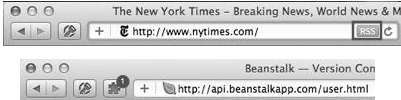
\includegraphics[scale=0.8]{images/rss_api.png}
        \caption{ The RSS discovery mechanism already present in modern browsers.}
        The toolbar button shows a badge with the number of resources found when visiting a site with embedded resource descriptions.
        \label{fig:rss_api}
\end{figure}

The following annotations for inter-links between services are defined to enable discovery:

\begin{enumerate}
\item {\it Link to Superclass}: When a resource is a subclass of another resource, this link is indicated by the rel attribute hresource-is-a. This implies that wherever the superclass is accepted, the subclass is also accepted. For e.g., if a publisher defines a Book resource to provide a search of their catalog, they could annotate the resource to be a subclass of a more generic Book resource.

\begin{minted}{html}
<a rel="hresource-is-a"
               href="http://dublincore.org/book/">
               Book
        </a>
\end{minted}

If there is another service from a bookshop that is known to accept a generic book resource for a purchase process, the client could infer that the specific book resource from the catalog would also be accepted there and use it.

For this linking to work properly, we need a core set of resources that can be extended by others. Fortunately, there is already a project named Dublin Core running that has defined many commonly used resources. We could reuse these resources for our purpose and use them as the root resources.

\item {\it Link to Consumers}: When an attribute of a service is consumed by another known service, this is annotated using \texttt{a rel attribute hresource-consumed-by}. This enables a software agent to find out what all can be done with the resource that it has already retrieved.

\begin{minted}{html}
<code class="attribute">
             ISBN
        </code>
        Consumers:
        <ul>
            <li rel="hresource-consumed-by">
               http://bookshop.com/book-order\#isbn
            </li>
            <li rel="hresource-consumed-by">
               http://library.com/rented-book\#isbn
            </li>
        </ul>
\end{minted}

\item {\it Link to Producers}: Similar to the link to consumers, services can annotate a link to a producer of one of its attributes. This helps reverse traversal of resources and also makes the system more peer-to-peer. This way, a link needs to be provided in either at one of the consumers or at the provider and an agent can identify this with link traversal. The annotation is made with the rel attribute \texttt{hresource-produced-by}.

\begin{figure}
        \centering
        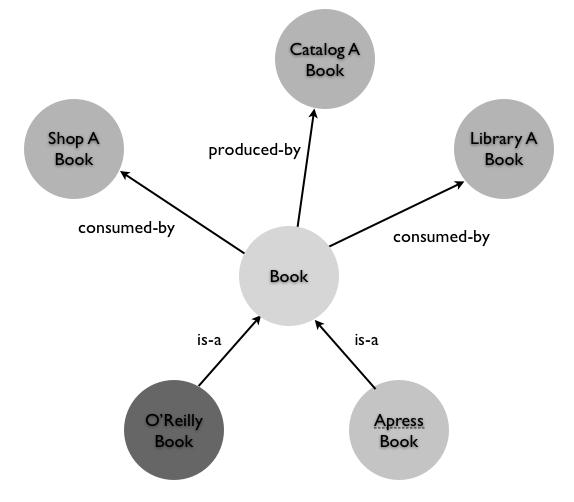
\includegraphics[scale=0.5]{images/res_graph.png}
        \caption{A graph constructed from the links between the resources.}
        \label{fig:res_graph}
\end{figure}

\section{Composition}

Service composition is made possible by using the same annotations that were made for discovery. A graph is constructed starting from a resource and then traversing the parent, consumer and producer links recursively. At each page, the descriptions are extracted and converted to RDF to update the graph. This way, a software agent that does not have the identifier or a search parameter to access a specific resource could traverse the graph to figure out what other information could be used to lookup the identifier and present the choice to the user.

For e.g., the service provided by a bookshop might need the ISBN to order a book. However, the traversal of the graph could reveal a catalog service that retrieves book resources using titles or author names. This allows the software agent to provide a choice to the user where he can enter either the ISBN or the title.

This works in the reverse direction also. Having received access to a resource, the software agent can suggest what all operations can accept the resource. So effectively a service that has a book resource can provide options for services from shops that let the user order the book or libraries that let the user lend the book .
\end{spacing}